% This LaTeX document needs to be compiled with XeLaTeX.
\documentclass[
  10
]{article}
\usepackage[margin=2cm,includehead=true,includefoot=true,centering,]{geometry}
\usepackage{xcolor}
\usepackage{ucharclasses}
\usepackage{hyperref}
\usepackage{amsmath,amssymb}
\usepackage{amsfonts}
\usepackage[version=4]{mhchem}
\usepackage{stmaryrd}
\usepackage{bbold}
\usepackage{polyglossia}
\usepackage{fontspec}
\usepackage{ctex}
\usepackage[export]{adjustbox}
\usepackage{tabularx}
\usepackage{booktabs}

\usepackage{setspace}
\setstretch{1.2}

\makeatletter
\@ifundefined{KOMAClassName}{% if non-KOMA class
  \IfFileExists{parskip.sty}{%
    \usepackage{parskip}
  }{% else
    \setlength{\parindent}{0pt}
    \setlength{\parskip}{6pt plus 2pt minus 1pt}}
}{% if KOMA class
  \KOMAoptions{parskip=half}}
\makeatother
\usepackage{longtable,booktabs,array}
\usepackage{multirow}
\usepackage{calc} % for calculating minipage widths
% Correct order of tables after \paragraph or \subparagraph
\usepackage{etoolbox}
\makeatletter
\patchcmd\longtable{\par}{\if@noskipsec\mbox{}\fi\par}{}{}
\makeatother
% Allow footnotes in longtable head/foot
\IfFileExists{footnotehyper.sty}{\usepackage{footnotehyper}}{\usepackage{footnote}}
\makesavenoteenv{longtable}
\usepackage{graphicx}
\makeatletter
\newsavebox\pandoc@box
\newcommand*\pandocbounded[1]{% scales image to fit in text height/width
  \sbox\pandoc@box{#1}%
  \Gscale@div\@tempa{\textheight}{\dimexpr\ht\pandoc@box+\dp\pandoc@box\relax}%
  \Gscale@div\@tempb{\linewidth}{\wd\pandoc@box}%
  \ifdim\@tempb\p@<\@tempa\p@\let\@tempa\@tempb\fi% select the smaller of both
  \ifdim\@tempa\p@<\p@\scalebox{\@tempa}{\usebox\pandoc@box}%
  \else\usebox{\pandoc@box}%
  \fi%
}
% Set default figure placement to htbp
\def\fps@figure{htbp}
\makeatother
\setlength{\emergencystretch}{3em} % prevent overfull lines
\providecommand{\tightlist}{%
  \setlength{\itemsep}{0pt}\setlength{\parskip}{0pt}}


\hypersetup{colorlinks=true, linkcolor=blue, filecolor=magenta, urlcolor=cyan,}
\urlstyle{same}

\usepackage{colortbl}
\definecolor{table-row-color}{HTML}{999999}
\definecolor{table-rule-color}{HTML}{999999}
%\arrayrulecolor{black!40}
\arrayrulecolor{table-rule-color}     % color of \toprule, \midrule, \bottomrule
\setlength{\aboverulesep}{0pt}
\setlength{\belowrulesep}{0pt}


\setotherlanguages{english}
\IfFontExistsTF{Source Han Serif CN}
{\newfontfamily\chinesefont{Source Han Serif CN}}
{\IfFontExistsTF{Noto Serif CJK SC}
  {\newfontfamily\chinesefont{Noto Serif CJK SC}}
  {\IfFontExistsTF{SimSun}
    {\newfontfamily\chinesefont{SimSun}}
    {\IfFontExistsTF{FangSong}
      {\newfontfamily\chinesefont{FangSong}}
      {\newfontfamily\chinesefont{Arial Unicode MS}}
}}}
\IfFontExistsTF{Times New Roman}
{\newfontfamily\englishfont{Times New Roman}}
{\IfFontExistsTF{Liberation Serif}
  {\newfontfamily\englishfont{Liberation Serif}}
  {\IfFontExistsTF{DejaVu Serif}
    {\newfontfamily\englishfont{DejaVu Serif}}
    {\newfontfamily\englishfont{Arial}}
}}


\author{}
\date{}

\begin{document}


A47备案号：

\section{MH}\label{mh}

\section{中华人民共和国民用航空行业标准}\label{ux4e2dux534eux4ebaux6c11ux5171ux548cux56fdux6c11ux7528ux822aux7a7aux884cux4e1aux6807ux51c6}

MH/T4016.9-2011

\section{民用航空气象第9部分：自动气象观测系统数据输出格式}\label{ux6c11ux7528ux822aux7a7aux6c14ux8c61ux7b2c9ux90e8ux5206ux81eaux52a8ux6c14ux8c61ux89c2ux6d4bux7cfbux7edfux6570ux636eux8f93ux51faux683cux5f0f}

Civil aviation meteorologyPart 9:Output message format of automated
weather observing system

\section{中国民用航空局
发布}\label{ux4e2dux56fdux6c11ux7528ux822aux7a7aux5c40-ux53d1ux5e03}

\section{前言}\label{ux524dux8a00}

MH/T4016《民用航空气象》分为以下部分：第1部分：观测和报告；第2部分：预报；第3部分：服务；第4部分：设备配备；第5部分：设备技术要求；第6部分：电码；第7部分：气候资料整编与分析；第8部分：天气图编绘与分析；第9部分：自动气象观测系统数据输出格式；第10部分：地面观测记录；

本部分为MH/T4016的第9部分。\\
本部分按照GB/T1.1一2009给出的规则起草。

本部分由中国民用航空局空中交通管理局提出并负责解释。

本部分由中国民用航空局航空器适航审定司批准立项。

本部分由中国民航科学技术研究院归口

本部分起草单位：中国民用航空局空中交通管理局、中国民用航空华北地区空中交通管理局、中国民用航空中南地区空中交通管理局。

本部分主要起草人：楚建杰、崔屹、郭翔、王新。

\section{民用航空气象}\label{ux6c11ux7528ux822aux7a7aux6c14ux8c61}

\section{第9部分：自动气象观测系统数据输出格式}\label{ux7b2c9ux90e8ux5206ux81eaux52a8ux6c14ux8c61ux89c2ux6d4bux7cfbux7edfux6570ux636eux8f93ux51faux683cux5f0f}

\section{1范围}\label{ux8303ux56f4}

MH/T4016的本部分规定了民用航空运输机场配备的自动气象观测系统的电子数据输出格式。\\
本部分适用于民用航空气象自动气象观测系统的电子数据的输出。

\section{2规范性引用文件}\label{ux89c4ux8303ux6027ux5f15ux7528ux6587ux4ef6}

下列文件对于本文件的应用是必不可少的。凡是注日期的引用文件，仅所注日期的版本适用于本文件。凡是不注日期的引用文件，其最新版本（包括所有的修改单）适用于本文件。

MH/T4016.1 民用航空气象 第1部分：观测和报告

\section{3术语和定义}\label{ux672fux8bedux548cux5b9aux4e49}

MH/T4016.1中界定的以及下列术语和定义适用于本文件。

3.1

消息 message自动气象观测系统数据流的一种表现形式。

\section{4消息}\label{ux6d88ux606f}

\section{4.1消息的组成}\label{ux6d88ux606fux7684ux7ec4ux6210}

4.1.1消息包含一个消息头域和数据部分，数据部分由1个或多个数据域构成。消息由ASCII字符串组成，用控制字符SOH、STX、ETX和EOT作为分隔符。

4.1.2控制字符的定义见表1。

表1控制字符

\begin{longtable}[]{@{}|l|l|@{}}
\toprule\noalign{}
\endhead
\bottomrule\noalign{}
\endlastfoot
\hline
名称 & 描述 \\
\hline
SOH & ASCII 0x01，表示一条新消息的开始，同时表示消息头域的开始。 \\
\hline
STX & ASCII0x02，表示一个新数据域的开始。 \\
\hline
ETX & ASCII0x03，表示消息头域或数据域的结束。 \\
\hline
EOT & ASCII0x04，表示消息的结束。 \\
\hline
\end{longtable}

\section{4.2消息的类型}\label{ux6d88ux606fux7684ux7c7bux578b}

根据内容，消息分为10类。表2定义了消息类型及对应的消息内容。

表2消息的类型

\begin{longtable}[]{@{}|l|l|l|@{}}
\toprule\noalign{}
\endhead
\bottomrule\noalign{}
\endlastfoot
\hline
序号 & 消息类型 & 消息内容 \\
\hline
1 & CLOUD & 云 \\
\hline
2 & HUMITEMP & 温度和湿度 \\
\hline
3 & PRESS & 大气压力 \\
\hline
4 & RAIN & 降水 \\
\hline
5 & VIS & 能见度和跑道视程 \\
\hline
6 & WIND & 风速和风向 \\
\hline
7 & PW & 天气现象 \\
\hline
8 & PV & 主导能见度 \\
\hline
9 & ROSA & 道面传感器 \\
\hline
10 & RWYLIGHTS & 跑道灯光 \\
\hline
\end{longtable}

\section{5消息头域}\label{ux6d88ux606fux5934ux57df}

5.1消息头域由6个子域和2个控制符构成。消息头域里的子域用``\textbar''（ASCII0x7C）字符分隔。\\
5.2表3定义了消息头域的结构。

表3消息头域

\begin{longtable}[]{@{}llll@{}}
\toprule\noalign{}
\endhead
\bottomrule\noalign{}
\endlastfoot
序号 & 子域和控制符 & 内容 & \\
1 & SOH & 控制符，ASCII0x01，表示一条新消息的开始，同时表示消息头域
的开始。 & \\
2 & Version & 消息版本号。 & \\
3 & Sequence number &
消息序列号。由5位数据位组成。在系统内部这个序列号是一个
16位的无符号整型数，取值范围是00001一65535。0值不可用。
如果序列号没有使用或为0值，则该域为空。 & \\
\multirow{2}{*}{4} & \multirow{2}{*}{Messagetime} &
消息被创建或被放入缓存以备发送的时间。使用协调世界时。
时间格式为ASCII格式的Unixtime。 & \\
& & 如果该域没有使用，则该域为空。 & \\
5 & Message type & 消息类型。定义了消息包含何种内容的数据，见表2。 & \\
\multirow{2}{*}{6} & \multirow{2}{*}{Sensor ID} &
传感器标志，定义了数据的来源。 & \\
& & 如果数据无法定位，则该域为空。 & \\
\multirow{2}{*}{7} & \multirow{2}{*}{Location ID} &
传感器位置标志，例：``02R''，``20L''。 & \\
& & 如果数据无法定位，则该域为空。如果位置信息不可用，这个域包
含3个斜线字符（///）。 & \\
\multicolumn{2}{@{}l}{%
8 ETX 控制符，ASCII0x04，表示消息的结束。} & \multicolumn{2}{l@{}}{%
} \\
\end{longtable}

示例1：\\
1\textbar00124\textbar1011173512\textbar VIS\textbar1\textbar02L\ldots data
part\ldots{}\\
示例2：\\
1/00124\textbar/VIS/1\textbar02L\ldots data part\ldots{}\\
示例3：\\
1\textbar\textbar vIS\textbar1/02L\ldots datapart\ldots{}\\
示例4：\\
1\textbar\textbar1011173512\textbar VIS\textbar1\textbar///\ldots datapart\ldots{}

\section{6数据部分}\label{ux6570ux636eux90e8ux5206}

\section{6.1数据域}\label{ux6570ux636eux57df}

6.1.1数据部分由一个或多个数据域构成，数据部分位于消息头域之后和消息结束分隔符（EOT）之前。数据部分内的每个数据域以STX开始，ETX结束，并且包含若干个子域。子域之间用分隔字符''\textbar``(ASCII
\(0 \mathbf { x } 7 \mathbf { C } )\) 分隔。\\
6.1.2表4定义了数据域的结构。

表4数据域结构

\begin{longtable}[]{@{}|l|l|l|@{}}
\toprule\noalign{}
\endhead
\bottomrule\noalign{}
\endlastfoot
\hline
序号 & 子域和控制符 & 描述 \\
\hline
1 & STX & 控制符，ASCII0x02，表示一个新数据域的开始。 \\
\hline
2 & Item name & 数据项的名称，例如，``VERVIS''，``CH1INS''等。 \\
\hline
3 & Data type &
数据类型：长整型（I），实型（R）或字符串型（S），见6.1.3。 \\
\hline
4 & Status & 数据状态，有以下几种取值：N，M，C，O，一，I,U，见6.1.4。 \\
\hline
5 & Value & 数据的值。 \\
\hline
6 & Unit &
数据单位（例如``米''，``米每秒''等）。如果数据无单位，该项为空。所有单位均为国际制单位。 \\
\hline
7 & ETX & 控制符，ASCII0x03，表示消息头域或数据域的结束。 \\
\hline
\end{longtable}

6.1.3数据的类型为以下几种：

数据类型I（长整型）是一个可变宽度数字，为32位符号整型；\\
数据类型R（实型）是一个可变宽度浮点数，在小数点左边应至少有一位，用``.''作为小数分隔符，小数点右边应至少有两位（例如1.23）；\\
数据类型S（字符串）是一个可变宽度字符串。该字符串以分隔符``\textbar''（ASCIIOx7C）结束，\textbar''字符不应包含在字符串中。

6.1.4数据的状态应使用一个状态编码来描述其有效性。数据的状态及其编码的定义见表5。

表5数据状态编码

\begin{longtable}[]{@{}|l|l|l|@{}}
\toprule\noalign{}
\endhead
\bottomrule\noalign{}
\endlastfoot
\hline
状态 & 编码 & 描述 \\
\hline
Normal & N & 数据来自于传感器并且是有效的。 \\
\hline
Manual & M & 数据是有效的，但是由观测员输人系统。 \\
\hline
Copied & C & 数据来自于备份传感器。 \\
\hline
Old & 0 & 数据到了某个超时阶段还未被更新，但仍然认为其是有效数据。 \\
\hline
Missing & &
数据还没有被更新并且已经认为丢失。丢失前的一段时间内，数据通常处于``old''状态。数据丢失
时Value用``///''表示。 \\
\hline
Invalid & I &
数据无效或超出范围，已经不能被使用。当传感器或数据线路故障时会发生这种情况。 \\
\hline
Undefined & U & 数据的值可能是有效的，但是不能被使用。 \\
\hline
\end{longtable}

\section{6.2数据更新时间}\label{ux6570ux636eux66f4ux65b0ux65f6ux95f4}

6.2.1每条消息应包含表明数据对象被系统更新的时间，该时间为协调世界时，以Unixtime时间格式表示。更新时间作为一个数据域居于消息头域之后，其他数据域之前。

示例：

1\textbar00125\textbar CL0UD\textbar1\textbar02L＜ETX\textgreater TIME\textbar I\textbar N\textbar1011098674\textbar{}
\(<\) ETX\textgreater otherfields.·6.2.2时间数据域的``单位''子域为空。

\section{6.3云消息数据部分的构成}\label{ux4e91ux6d88ux606fux6570ux636eux90e8ux5206ux7684ux6784ux6210}

云消息数据部分的构成见表6，表中某个域可能没有。

表6云（CLOUD）消息的数据域

\begin{longtable}[]{@{}|l|l|l|l|l|@{}}
\toprule\noalign{}
\endhead
\bottomrule\noalign{}
\endlastfoot
\hline
序号 & 名称 & 类型 & 单位 & 描述 \\
\hline
1 & TIME & I & & 数据更新时间（Unixtime，协调世界时） \\
\hline
2 & ISSKYCLEAR & I & & 标志：是否是晴空 0---非晴空 1-晴空 \\
\hline
3 & ISVERVIS & I & & 标志：是否探测到垂直能见度 0---未探测到垂直能见度
---探测到垂直能见度 \\
\hline
4 & VERVIS & R & m & 垂直能见度值 \\
\hline
5 & CLOUDBASE & R & m & 云底高度 \\
\hline
6 & CH1INS & R & m & 第一层云高 \\
\hline
7 & CH2INS & R & m & 第二层云高 \\
\hline
8 & CH3INS & R & m & 第三层云高 \\
\hline
9 & *AMOUNT1 & S & & 天空状况数据中的第一层云量（八进制） \\
\hline
\end{longtable}

表6（续）

\begin{longtable}[]{@{}|l|l|l|l|l|@{}}
\toprule\noalign{}
\endhead
\bottomrule\noalign{}
\endlastfoot
\hline
序号 & 名称 & 类型 & 单位 & 描述 \\
\hline
10 & *CH1 & R & m & 天空状况数据中的第一层云高 \\
\hline
11 & *AMOUNT2 & S & & 天空状况数据中的第二层云量（八进制） \\
\hline
12 & *CH2 & R & m & 天空状况数据中的第二层云高 \\
\hline
13 & *AMOUNT3 & S & 一 & 天空状况数据中的第三层云量（八进制） \\
\hline
14 & *CH3 & R & m & 天空状况数据中的第三层云高 \\
\hline
15 & *AMOUNT4 & s & 一 & 天空状况数据中的第四层云量（八进制） \\
\hline
16 & *CH4 & R & m & 天空状况数据中的第四层云高 \\
\hline
\end{longtable}

注：本表格中带 \(^ { \ast }\)
的数据域是依据特定算法估算得到的，仅供参考。

\section{示例：}\label{ux793aux4f8b}

1\textbar00125\textbar CL0UD\textbar1\textbar04LTIME\textbar I\textbar N\textbar1011098674\textbar ISSKYCLEAR\textbar I\textbar N\textbar O\textbar ISVERVIS\textbar I\textbar N\textbar1\textbar VERVIS\textbar R\textbar N\textbar180.00\textbar mCLOUDBASE\textbar R\textbar U\textbar///\textbar mCH1INS\textbar R\textbar U丨///\textbar mCH2INS\textbar R\textbar U\textbar///\textbar mCH3INS\textbar R\textbar U\textbar///\textbar mAMOUNT1\textbar I\textbar N\textbar1\textbar CH1\textbar R\textbar N\textbar1300\textbar mAMOUNT2\textbar I\textbar N\textbar4\textbar CH2\textbar R\textbar N\textbar2200\textbar mAMOUNT3\textbar I\textbar N\textbar8\textbar CH3\textbar R\textbar N\textbar7000\textbar mAMOUNT4\textbar I\textbar N\textbar0\textbar CH4\textbar R\textbar-\textbar///\textbar m注：为了便于阅读，将一条消息分行显示

\section{6.4温湿度消息数据部分的构成}\label{ux6e29ux6e7fux5ea6ux6d88ux606fux6570ux636eux90e8ux5206ux7684ux6784ux6210}

温湿度消息数据部分的构成见表7，表中某个域可能没有。

表7 温湿度（HUMITEMP）消息的数据域

\begin{longtable}[]{@{}|l|l|l|l|l|@{}}
\toprule\noalign{}
\endhead
\bottomrule\noalign{}
\endlastfoot
\hline
序号 & 名称 & 类型 & 单位 & 描述 \\
\hline
1 & TIME & I & & 数据更新时间（Unixtime，协调世界时） \\
\hline
2 & TAINS & R & C & 瞬时温度 \\
\hline
3 & TA10M & R & C & 10min最低温度（瞬时值） \\
\hline
\end{longtable}

MH/T4016.9-2011

表7（续）

\begin{longtable}[]{@{}|l|l|l|l|l|@{}}
\toprule\noalign{}
\endhead
\bottomrule\noalign{}
\endlastfoot
\hline
序号 & 名称 & 类型 & 单位 & 描述 \\
\hline
4 & TA10X & R & C & 10min最高温度（瞬时值） \\
\hline
5 & TA1hA & R & C & 1h平均温度 \\
\hline
6 & TA1hM & R & C & 1h最低温度（瞬时值） \\
\hline
7 & TA1hX & R & C & 1h最高温度（瞬时值） \\
\hline
8 & TDINS & R & C & 瞬时露点值 \\
\hline
9 & RHINS & R & \% & 瞬时相对湿度 \\
\hline
10 & VPINS & R & hPa & 瞬时水汽压 \\
\hline
\multicolumn{5}{@{}l@{}}{%
注：在单位一项中C表示摄氏度。} \\
\hline
\end{longtable}

\section{示例：}\label{ux793aux4f8b-1}

1\textbar00126\textbar HUMITEMP\textbar1\textbar CWTIME\textbar I\textbar N\textbar1011098674\textbar TAINS\textbar R\textbar N\textbar20.0O\textbar CTA10M\textbar R\textbar N\textbar20.00\textbar CTA10X\textbar R\textbar N\textbar20.00\textbar CTA1hA\textbar R\textbar N\textbar20.00\textbar CTA1hM\textbar R\textbar N\textbar20.00\textbar CTA1hX\textbar R\textbar N\textbar20.00\textbar CTDINS\textbar R\textbar N\textbar13.55\textbar CRHINS\textbar R\textbar N\textbar66.0O\textbar\%VPINS\textbar R\textbar N\textbar15.76\textbar hPa注：为了便于阅读，将一条消息分行显示。

\section{6.5
气压消息数据部分的构成}\label{ux6c14ux538bux6d88ux606fux6570ux636eux90e8ux5206ux7684ux6784ux6210}

气压消息数据部分的构成见表8，表中某个域可能没有。

表8 气压（PRESS）消息的数据域

\begin{longtable}[]{@{}|l|l|l|l|l|@{}}
\toprule\noalign{}
\endhead
\bottomrule\noalign{}
\endlastfoot
\hline
序号 & 名称 & 类型 & 单位 & 描述 \\
\hline
1 & TIME & I & 一 & 数据更新时间（Unixtime，协调世界时） \\
\hline
2 & PAINS & R & hPa & 瞬时气压 \\
\hline
3 & QFEINS & R & hPa & 瞬时场面气压（QFE） \\
\hline
4 & QFEM & R & hPa & 10min最小场压（最小瞬时值） \\
\hline
5 & QFEX & R & hPa & 10min最大场压（最大瞬时值） \\
\hline
6 & QFFINS & R & hPa & 瞬时QFF \\
\hline
7 & QNHINS & R & hPa & 瞬时修正海平面气压（QNH） \\
\hline
8 & QFESYNOP & R & hPa & 与陆地测站地面天气报告（SYNOP）相关的QFE；
如果做了配置，将SYNOP的高度从传感器高度中减去。 \\
\hline
\end{longtable}

表8（续）

\begin{longtable}[]{@{}|l|l|l|l|l|@{}}
\toprule\noalign{}
\endhead
\bottomrule\noalign{}
\endlastfoot
\hline
序号 & 名称 & 类型 & 单位 & 描述 \\
\hline
9 & QFESYNOPT & & & 与SYNOP相关的QFE趋势，取值范围为整数0到8，包
括0和8。 \\
\hline
10 & QFESYNOP3H & R & hPa &
QFE3h变化，即：当前值与3h前的值之间的差异。 \\
\hline
11 & FL & I & 一 & 过渡层，从QNHINS计算而来。 \\
\hline
12 & ALT & I & m & 过渡层海拔高度。 \\
\hline
\multicolumn{5}{@{}l@{}}{%
注：QFF表示按实际大气状态换算至海平面的气压值。} \\
\hline
\end{longtable}

\section{示例：}\label{ux793aux4f8b-2}

1\textbar00127\textbar\textbar PRESS\textbar1\textbar02L\\
TIME\textbar I\textbar N\textbar1011101296\textbar{}\\
PAINS\textbar R\textbar N\textbar988.78\textbar hPa\\
QFEINS\textbar R\textbar N\textbar988.82\textbar hPaQFEM\textbar R\textbar N\textbar988.82\textbar hPa\\
QFEX\textbar R\textbar N\textbar1006.30\textbar hPa\\
QFFINS\textbar R\textbar N\textbar989.56\textbar hPaQNHINS\textbar R\textbar N\textbar989.58\textbar hPaQFESYNOP\textbar R\textbar N\textbar988.82\textbar hPaQFESYNOPT\textbar I\textbar N\textbar3\textbar{}\\
QFFSYNOP3H\textbar R\textbar N\textbar27.20\textbar hPaFL\textbar I\textbar N\textbar35\textbar{}\\
ALT\textbar I\textbar N\textbar3344\textbar m\\
\strut \\
注：为了便于阅读，将一条消息分行显示。

\section{6.6
降水消息数据部分的构成}\label{ux964dux6c34ux6d88ux606fux6570ux636eux90e8ux5206ux7684ux6784ux6210}

降水消息数据部分的构成见表9，表中某个域可能没有。

表9 降水（RAIN）消息数据域

\begin{longtable}[]{@{}|l|l|l|l|l|@{}}
\toprule\noalign{}
\endhead
\bottomrule\noalign{}
\endlastfoot
\hline
序号 & 名称 & 类型 & 单位 & 描述 \\
\hline
1 & TIME & I & & 数据更新时间（Unixtime，协调世界时） \\
\hline
2 & RAINON & I & & 降水传感器是否探测到降水： 0------没探测到降水
非0---探测到降水 \\
\hline
3 & DURATION\_1H & R & min & 最近60min内的降水持续时间 \\
\hline
4 & AMOUNT\_INS & R & mm &
从降水传感器得到的瞬时降水量（时间范围取决于传感器配置） \\
\hline
5 & SUM\_INS & R & mm &
从降水传感器得到的瞬时总降水量（时间范围取决于传感器配置） \\
\hline
6 & SUM\_1H & R & mm & 最近60min的总降水量 \\
\hline
\end{longtable}

MH/T4016.9-2011

\section{示例：}\label{ux793aux4f8b-3}

SOH \(>\) 1\textbar00128\textbar\textbar RAIN\textbar1\textbar CW \(<\)
ETX\textgreater TIME\textbar I\textbar N\textbar1011098674\textbar RAINON\textbar IN\textbar1\textbar STX\textgreater DURATION\_1H\textbar R\textbar N\textbar36.00\textbar STX\textgreater AMOUNT
INS\textbar R\textbar N\textbar2.0O\textbar mmSUM\_INS\textbar RN\textbar32.0O\textbar mmSUM\_1H\textbar R\textbar N\textbar65.00\textbar mm注：为了便于阅读，将一条消息分行显示。

\section{6.7能见度和跑道视程消息数据部分的构成}\label{ux80fdux89c1ux5ea6ux548cux8dd1ux9053ux89c6ux7a0bux6d88ux606fux6570ux636eux90e8ux5206ux7684ux6784ux6210}

能见度和跑道视程消息数据部分的构成见表10，表中某个域可能没有。

表10能见度和跑道视程（VIS）消息数据域

\begin{longtable}[]{@{}|l|l|l|l|l|@{}}
\toprule\noalign{}
\endhead
\bottomrule\noalign{}
\endlastfoot
\hline
序号 & 名称 & 类型 & 单位 & 描述 \\
\hline
1 & TIME & I & 一 & 数据更新时间（Unixtime，协调世界时） \\
\hline
2 & RawRVR & I & m & 原始跑道视程（RVR）瞬时值 \\
\hline
3 & RVR & I & m & RVR瞬时值 \\
\hline
4 & RVR1A & I & m & RVR1min平均值 \\
\hline
5 & RVR1A10M & I & m & 最近10min内的最小1min平均值 \\
\hline
6 & RVR1A10X & I & m & 最近10min内的最大1min平均值 \\
\hline
7 & RVR2A & I & m & RVR2min平均值 \\
\hline
8 & RVR10A & I & m & RVR10min平均值 \\
\hline
9 & RVR10M & I & m & RVR10min最小值（最小瞬时值） \\
\hline
10 & RVR10X & I & m & RVR10min最大值（最大瞬时值） \\
\hline
11 & RVR10T & I & & RVR10min趋势： -1------减小 0---无趋势 1-增加 \\
\hline
12 & RawMOR & R & m & 原始瞬时气象光学视程（MOR） \\
\hline
13 & MOR & R & m & 瞬时MOR \\
\hline
14 & MOR1A & I & m & MOR1min平均值 \\
\hline
15 & MOR2A & I & m & MOR2min平均值 \\
\hline
16 & MOR10A & I & m & MOR10min平均值 \\
\hline
17 & MOR10M & I & m & MOR10min最小值（最小瞬时值） \\
\hline
18 & MOR10X & I & m & MOR10min最大值（最大瞬时值） \\
\hline
19 & VIS1K & R & m & 1000cd亮度计算出的能见度 \\
\hline
20 & RawVIS & R & m & 原始VIS瞬时值 \\
\hline
\end{longtable}

表10（续）

\begin{longtable}[]{@{}|l|l|l|l|l|@{}}
\toprule\noalign{}
\endhead
\bottomrule\noalign{}
\endlastfoot
\hline
序号 & 名称 & 类型 & 单位 & 描述 \\
\hline
21 & VIS & R & m & 瞬时能见度值 \\
\hline
22 & VIS1A & I & m & 能见度1min平均值 \\
\hline
23 & VIS2A & I & m & 能见度2min平均值 \\
\hline
24 & VIS10A & & m & 能见度10min平均值 \\
\hline
25 & VIS10M & i & m & 能见度10min最小值（最小瞬时值） \\
\hline
26 & VIS10X & I & m & 能见度10min最大值（最大瞬时值） \\
\hline
27 & BL & R & cdm2 & 背景亮度瞬时值（cd/m） \\
\hline
28 & BL1A & R & cdm2 & 背景亮度1min平均值（cd/m） \\
\hline
29 & BL2A & R & cdm2 & 背景亮度2min平均值（cd/m） \\
\hline
30 & LIGHTS & R & \% & 跑道灯光设置 \\
\hline
31 & EDGELIGHTS & R & \% & 跑道边灯灯光设置 \\
\hline
32 & CENTERLIGHTS & R & \% & 跑道中线灯灯光设置 \\
\hline
\end{longtable}

\section{示例：}\label{ux793aux4f8b-4}

1\textbar00130\textbar\textbar VIS\textbar1\textbar02LTIME\textbar I\textbar N\textbar1011098674\textbar RawRVR\textbar I\textbar N\textbar695\textbar mRVR\textbar I\textbar N\textbar675\textbar mRVR1A\textbar I\textbar N\textbar675\textbar mRVR1A10M\textbar I\textbar N\textbar400\textbar mRVR1A10X\textbar I\textbar N\textbar675\textbar mRVR2A\textbar I\textbar N\textbar675\textbar mRVR10A\textbar I\textbar N\textbar650\textbar mRVR10M\textbar I\textbar N\textbar600\textbar mRVR10X\textbar I\textbar N\textbar675\textbar mRVR10T\textbar I\textbar N\textbar1\textbar RaWMOR\textbar R\textbar N\textbar400.00\textbar mMOR\textbar R\textbar N\textbar400.00\textbar mMOR1A\textbar I\textbar N\textbar350\textbar mMOR2A\textbar I\textbar N\textbar350\textbar mMOR10A\textbar I\textbar N\textbar300\textbar mMOR10M\textbar I\textbar N\textbar200\textbar mMOR10X\textbar I\textbar N\textbar400\textbar mVIS1K\textbar R\textbar N\textbar627.00\textbar mRawVIS\textbar R\textbar N\textbar627.00\textbar mVIS\textbar R\textbar N\textbar600.00\textbar mVIS1A\textbar I\textbar N\textbar600\textbar mVIS2A\textbar I\textbar N\textbar600\textbar mVIS10A\textbar I\textbar N\textbar500\textbar mVIS10M\textbar I\textbar N\textbar400\textbar mVIS10X\textbar I\textbar N\textbar600\textbar mBL\textbar R\textbar N\textbar456.00\textbar cdm2BL1A\textbar R\textbar N\textbar456.00\textbar cdm2BL2A\textbar R\textbar N\textbar456.00\textbar cdm2LIGHTS\textbar R\textbar N\textbar30.00\textbar\%EDGELIGHTS\textbar R\textbar N\textbar30.00\textbar\%CENTERLIGHTS\textbar R\textbar N\textbar30.0O\textbar 注：为了便于阅读，将一条消息分行显示。

\section{6.8风消息数据部分的构成}\label{ux98ceux6d88ux606fux6570ux636eux90e8ux5206ux7684ux6784ux6210}

风消息数据部分的构成见表11，表中某个域可能没有。

表11风（WIND）消息数据域

\begin{longtable}[]{@{}|l|l|l|l|l|@{}}
\toprule\noalign{}
\endhead
\bottomrule\noalign{}
\endlastfoot
\hline
序号 & 名称 & 类型 & 单位 & 描述 \\
\hline
1 & TIME & I & 一 & 数据更新时间（Unixtime，协调世界时） \\
\hline
2 & WSINS & R & mps & 瞬时风速 \\
\hline
3 & WDINS & I & deg & 瞬时风向 \\
\hline
4 & WS2A & R & mps & 风速2min平均值 \\
\hline
5 & WS2M & R & mps & 风速2min最小值 \\
\hline
6 & WS2X & R & mps & 风速2min最大值 \\
\hline
7 & WD2A & I & deg & 风向2min平均值 \\
\hline
8 & WD2M & I & deg & 风向2min最小值（按顺时针方向确定） \\
\hline
9 & WD2X & I & deg & 风向2min最大值（按顺时针方向确定） \\
\hline
10 & WS10A & R & mps & 风速10min平均值 \\
\hline
11 & WS10M & R & mps & 风速10min最小值 \\
\hline
12 & WS10X & R & mps & 风速10min最大值 \\
\hline
13 & WD10A & I & deg & 风向10min平均值 \\
\hline
14 & WD10M & i & deg & 风向10min最小值 \\
\hline
15 & WD10X & I & deg & 风向10min最大值 \\
\hline
16 & HW2A & R & mps & WS2A头风分量： 正头风 负---尾风 \\
\hline
17 & CW2A & R & mps & WS2A侧风分量： 正右 负左 \\
\hline
\end{longtable}

表11（续）

\begin{longtable}[]{@{}|l|l|l|l|l|@{}}
\toprule\noalign{}
\endhead
\bottomrule\noalign{}
\endlastfoot
\hline
序号 & 名称 & 类型 & 单位 & 描述 \\
\hline
18 & CW2A\_KT\_STR & S & &
字符串形式的侧风风速{[}以节（kn）为单位{]}，例如： L16--16kn左侧风
R08-8kn右侧风 \\
\hline
19 & CW2A\_MPS\_STR & S & & 字符串形式的侧风风速（以mps为单位），例如：
L08-8mps左侧风 R04-\/---4mps右侧风 \\
\hline
\multicolumn{5}{@{}l@{}}{%
} \\
\hline
\end{longtable}

\section{示例：}\label{ux793aux4f8b-5}

1\textbar00129\textbar\textbar WIND\textbar1\textbar02LTIME\textbar I\textbar N\textbar1011098674\textbar WSINS\textbar R\textbar N\textbar20.50\textbar mpsWDINS\textbar I\textbar N\textbar45\textbar degWS2A\textbar R\textbar N\textbar13.96\textbar mpsWS2M\textbar R\textbar N\textbar10.50\textbar mpsWS2X\textbar R\textbar N\textbar20.50\textbar mpsWD2A\textbar I\textbar N\textbar45\textbar degWD2M\textbar I\textbar N\textbar45\textbar degWD2X\textbar I\textbar N\textbar45\textbar degWS10A\textbar R\textbar N\textbar13.71\textbar mpsWS10M\textbar R\textbar N\textbar10.50\textbar mpsWS10X\textbar R\textbar N\textbar20.50\textbar mpsETX\textgreater WD10A\textbar I\textbar N\textbar45\textbar degWD10M\textbar I\textbar N\textbar45\textbar degWD10X\textbar I\textbar N\textbar45\textbar degHW2A\textbar R\textbar N\textbar9.87\textbar mpsCW2A\textbar R\textbar N\textbar9.87\textbar mpsCW2A\_KT\_STR\textbar S\textbar N\textbar R19\textbar CW2A\_MPS\_STR\textbar S\textbar N\textbar R10\textbar 注：为了便于阅读，将一条消息分行显示

\section{6.9天气现象消息数据部分的构成}\label{ux5929ux6c14ux73b0ux8c61ux6d88ux606fux6570ux636eux90e8ux5206ux7684ux6784ux6210}

天气现象消息数据部分的构成见表12，表中某个域可能没有。

表12 天气现象（PW）消息数据域

\begin{longtable}[]{@{}|l|l|l|l|l|l|@{}}
\toprule\noalign{}
\endhead
\bottomrule\noalign{}
\endlastfoot
\hline
序号 & 名称 & 类型 & 单位 & 描述 & \\
\hline
1 & TIME & I & & 数据更新时间（Unixtime，协调世界时） & \\
\hline
2 & PW & S & 一 & 瞬时电码格式的机场例行天气报告（METAR）天气代码 & \\
\hline
3 & RW & S & & 近时METAR天气代码，使用RE标准 & \\
\hline
\end{longtable}

表12（续）

\begin{longtable}[]{@{}|l|l|l|l|l|@{}}
\toprule\noalign{}
\endhead
\bottomrule\noalign{}
\endlastfoot
\hline
序号 & 名称 & 类型 & 单位 & 描述 \\
\hline
4 & WXNWS & S & 一 & 瞬时天气，美国国家气象局（NWS）代码 \\
\hline
5 & WMOINS & I & 一 & 瞬时天气，世界气象组织（WMO）代码 \\
\hline
6 & WMO15A & I & 一 & 15min天气，WMO代码 \\
\hline
7 & WMO60A & I & 一 & 60min天气，WMO代码 \\
\hline
8 & PRW1A & R & mmh & 1min平均降水强度 \\
\hline
9 & PRWS & R & mm & 累积降水总量 \\
\hline
10 & PRSS & R & mm & 累积降雪总量 \\
\hline
11 & TBINS & R & C & 瞬时表面温度 \\
\hline
\multicolumn{5}{@{}l@{}}{%
注：在单位域中mmh表示mm/h。} \\
\hline
\end{longtable}

\section{示例：}\label{ux793aux4f8b-6}

1\textbar00126\textbar\textbar PW\textbar1\textbar04L\\
TIME\textbar I\textbar N\textbar1011098674\textbar{}\\
PW\textbar S\textbar N\textbar-RA\textbar{}\\
RW\textbar S\textbar N\textbar RERA\textbar{}\\
WXNWS\textbar S\textbar N\textbar L\textbar{}\\
WMOINS\textbar I\textbar N\textbar52\textbar{}\\
WMO15A\textbar I\textbar N\textbar61\textbar{}\\
WMO60A\textbar I\textbar N\textbar61\textbar{}\\
PRW1A\textbar R\textbar N\textbar0.33\textbar mmh\\
PRWS\textbar R\textbar N\textbar2.10\textbar mm\\
PRSS\textbar R\textbar N\textbar1.20\textbar mm\\
TBINS\textbar R\textbar N\textbar23.40\textbar C\\
\strut \\
注：为了便于阅读，将一条消息分行显示

\section{6.10
主导能见度消息数据部分的构成}\label{ux4e3bux5bfcux80fdux89c1ux5ea6ux6d88ux606fux6570ux636eux90e8ux5206ux7684ux6784ux6210}

主导能见度消息数据部分的构成见表13，表中某个域可能没有。

表13 主导能见度（PV）消息数据域

\begin{longtable}[]{@{}|l|l|l|l|l|@{}}
\toprule\noalign{}
\endhead
\bottomrule\noalign{}
\endlastfoot
\hline
序号 & 名称 & 类型 & 单位 & 描述 \\
\hline
1 & TIME & I & 一 & 数据更新时间（Unixtime，协调世界时） \\
\hline
2 & RawVIS & R & m & 原始主导能见度瞬时值 \\
\hline
3 & VIS & R & m & 瞬时主导能见度 \\
\hline
4 & VIS1A & I & m & 主导能见度1min平均值 \\
\hline
5 & VIS2A & I & m & 主导能见度2min平均值 \\
\hline
6 & VIS10A & I & m & 主导能见度10min平均值 \\
\hline
7 & VIS10M & I & m & 主导能见度10min最小值（最小瞬时值） \\
\hline
\end{longtable}

表13（续）

\begin{longtable}[]{@{}|l|l|l|l|l|@{}}
\toprule\noalign{}
\endhead
\bottomrule\noalign{}
\endlastfoot
\hline
序号 & 名称 & 类型 & 单位 & 描述 \\
\hline
8 & VIS10X & I & m & 主导能见度10min最大值（最大瞬时值） \\
\hline
9 & SENSOR\_VIS10M & I & m & 在10min内一组数据的最小瞬时能见度值 \\
\hline
10 & SENSOR\_VIS10M\_DIR & S & & 在10min内最小瞬时能见度值的方向 \\
\hline
11 & SENSOR\_VIS10X & I & m & 在10min内一组数据的最大瞬时能见度值 \\
\hline
12 & SENSOR\_VIS10X\_DIR & S & & 在10min内最大瞬时能见度值的方向 \\
\hline
\multicolumn{5}{@{}l@{}}{%
注：本表格中的主导能见度是依据主导能见度的定义利用自动气象观测系统的数据计算得到的，仅供参考。} \\
\hline
\end{longtable}

\section{示例：}\label{ux793aux4f8b-7}

1\textbar00130\textbar\textbar PV\textbar1\textbar ACTIVE
TIME\textbar I\textbar N\textbar1011098674\textbar{}
RawVIS\textbar R\textbar N\textbar627.00\textbar m
VIS\textbar I\textbar N\textbar600\textbar m
VIS1A\textbar I\textbar N\textbar600\textbar m
VIS2A\textbar I\textbar N\textbar600\textbar m
VIS10A\textbar I\textbar N\textbar500\textbar m
VIS10M\textbar I\textbar N\textbar400\textbar m
VIS10X\textbar I\textbar N\textbar600\textbar m
SENSOR\_VIS10M\textbar I\textbar N\textbar45\textbar m
SENSOR\_VIS1OM\_DIR\textbar S\textbar N\textbar SE\textbar{}
SENSOR\_VIS10X\textbar I\textbar N\textbar7000\textbar m
SENSOR\_VIS1OX\_DIR\textbar S\textbar N\textbar W\textbar{}
注：为了便于阅读，将一条消息分行显示。

\section{6.11道面状况消息数据部分的构成}\label{ux9053ux9762ux72b6ux51b5ux6d88ux606fux6570ux636eux90e8ux5206ux7684ux6784ux6210}

道面状况消息数据部分的构成见表14，表中某个域可能没有。

表14 道面状况（ROSA）消息数据域

\begin{longtable}[]{@{}|l|l|l|l|l|@{}}
\toprule\noalign{}
\endhead
\bottomrule\noalign{}
\endlastfoot
\hline
序号 & 名称 & 类型 & 单位 & 描述 \\
\hline
1 & TIME & I & 一 & 数据更新时间（Unixtime，协调世界时） \\
\hline
2 & STEMP & R & C & 表面温度 \\
\hline
3 & GTEMP & R & C & 地温 \\
\hline
4 & SURFSTA & I & 一 & 表面状态 \\
\hline
5 & ALARM\_STATUS & S & & 告警状态 \\
\hline
6 & RAIN\_STATUS & S & & 雨状态 \\
\hline
7 & SURFACE\_STATUS & S & & 表面状态 \\
\hline
\end{longtable}

示例： 1\textbar19353\textbar1282788660\textbar R0SA\textbar1\textbar20R
TIME\textbar I\textbar N\textbar1282788660\textbar{}

STEMP\textbar R\textbar N\textbar52.70\textbar C\\
GTEMP\textbar R\textbar N\textbar38.60\textbar{} \(c <\)
ETX\textgreater{}\\
SURFSTAIN\textbar31\textbar{}\\
ALARM\_STATUS\textbar S\textbar N\textbar NO WARNINGETX\textgreater RAIN
STATUSSNCLEARETX\textgreater{}\\
STX\textgreater SURFACE\_STATUS\textbar S\textbar NDRYETX\textgreater{}\\
\strut \\
注：为了便于阅读，将一条消息分行显示。

\section{6.12
跑道灯光消息数据部分的构成}\label{ux8dd1ux9053ux706fux5149ux6d88ux606fux6570ux636eux90e8ux5206ux7684ux6784ux6210}

跑道灯光消息数据部分的构成见表15，表中某个域可能没有。

表15 跑道灯光（RWYLIGHTS）消息数据域

\begin{longtable}[]{@{}|l|l|l|l|l|@{}}
\toprule\noalign{}
\endhead
\bottomrule\noalign{}
\endlastfoot
\hline
序号 & 名称 & 类型 & 单位 & 描述 \\
\hline
1 & TIME & I & & 数据更新时间（Unixtime，协调世界时） \\
\hline
2 & LIGHTS & R & & 跑道灯光强度（\%） \\
\hline
3 & ISMANUAL & I & 一 & 是否人工输入，0 否，1---是 \\
\hline
4 & INFO & s & & 信息 \\
\hline
5 & 02L\_InUse & I & 一 & 02L跑道是否在用（灯光开启），0 否，1-是 \\
\hline
6 & 20R\_InUse & I & & 20R跑道是否在用（灯光开启），0 否，1---是 \\
\hline
\end{longtable}

\section{示例：}\label{ux793aux4f8b-8}

SOH\textgreater1\textbar19355\textbar1282788660\textbar RWYLIGHTS\textbar1\textbar WEST\\
TIME\textbar I\textbar N\textbar1282788660\textbar{}\\
LIGHTS\textbar R\textbar N\textbar10.00\textbar{}\\
ISMANUAL\textbar I\textbar N\textbar0\textbar{}\\
INFO\textbar S\textbar N\textbar Missing input data,using Default
Intensity\textbar{}\\
02L\_InUse\textbar I\textbar O\textbar0\textbar{}\\
20R\_InUse\textbar I\textbar0\textbar1\textbar{}\\
注1：消息头域中的``WEST''指跑道编号。\\
注2：为了便于阅读，将一条消息分行显示。

\pandocbounded{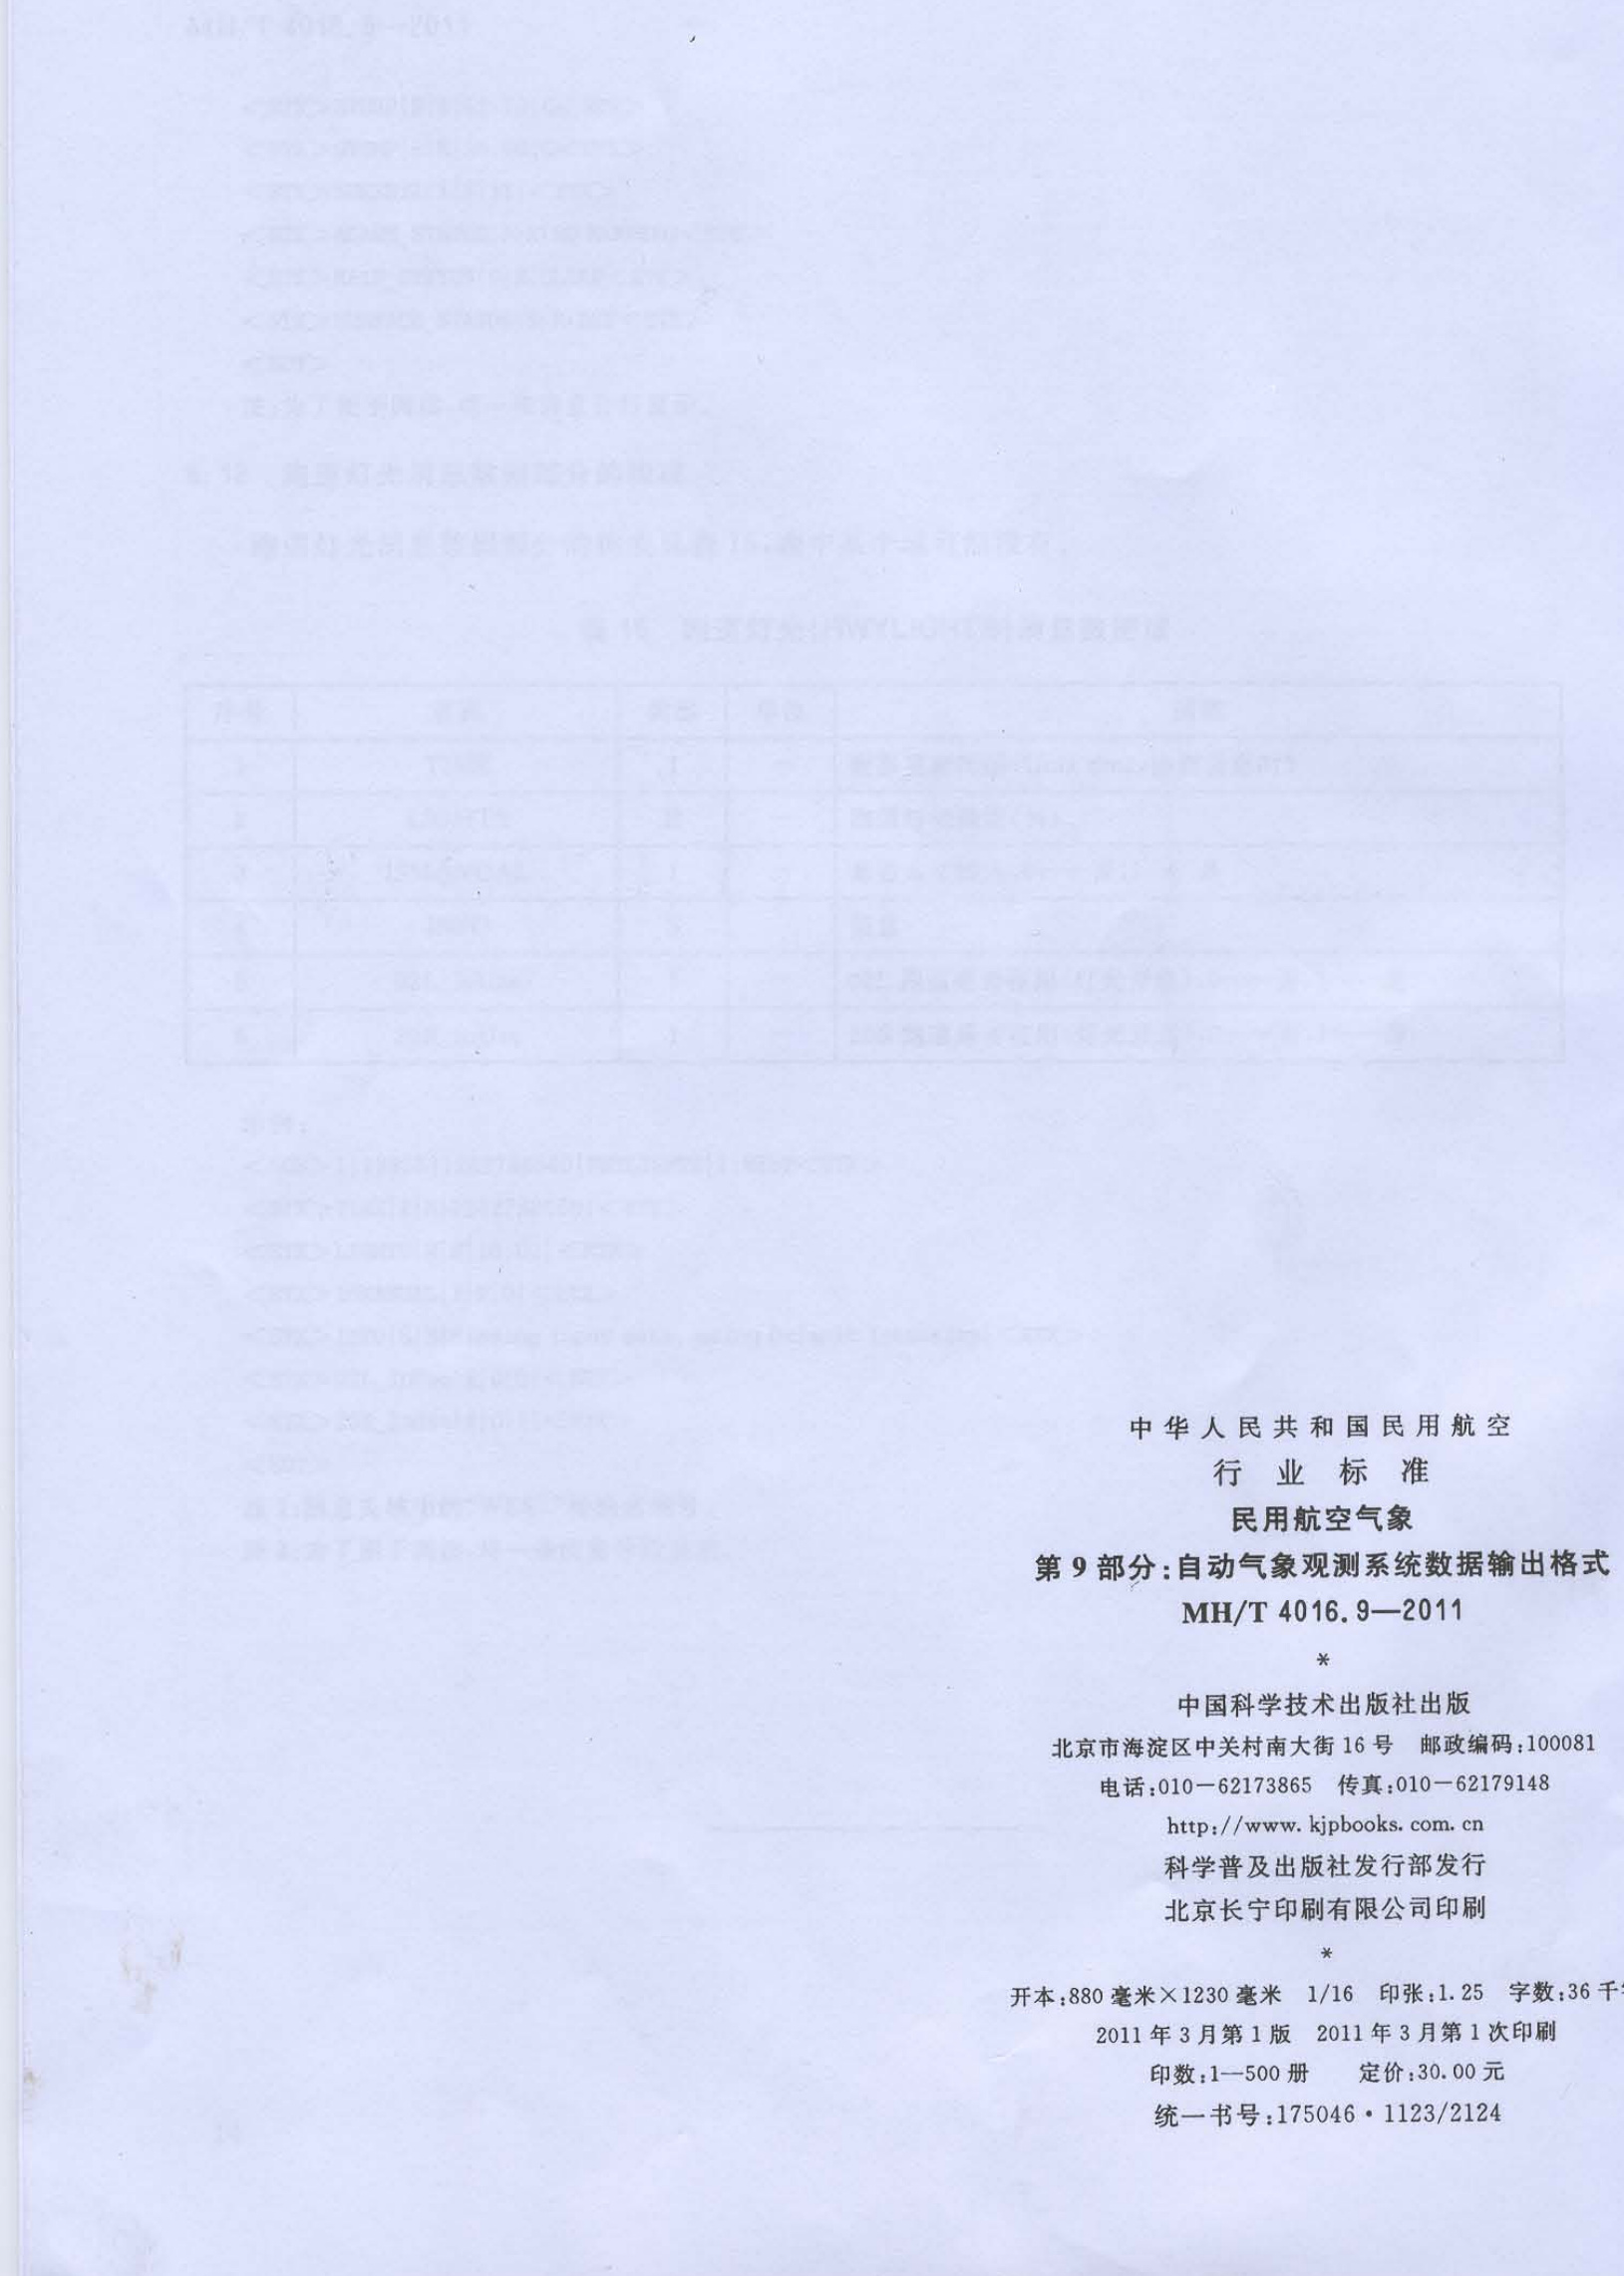
\includegraphics[keepaspectratio]{images/33d9869eaa89a3084e326eec29833fd038f638f83d64082142854eb76160d932.jpg}}

\end{document}
